\chapter{Ξεκινώντας στο Pygame}
\label{chap:pygame-intro}
%
\section{Εισαγωγή}
%
Μέχρι τώρα σας έχουμε δείξει απλά παιχνίδια που θα μπορούσατε κάλλιστα να παίζατε σε ένα τερματικό του PDP11! Πρέπει να ομολογήσουμε ότι στις μέρες μας ένα adventure κειμένου δεν θα είχε και μεγάλη τύχη στην αγορά. Καταλαβαίνετε βέβαια ότι αυτή η εισαγωγή ήταν απαραίτητη για να μάθετε τα βασικά της python και φυσικά για να ενεργοποιήσουμε την αλγοριθμική σας σκέψη! Πιστεύουμε ότι αυτό το καταφέραμε με το text adventure.

Είναι προφανές (τουλάχιστον σε μας) ότι δεν θα μπορούσαμε να ξεκινήσουμε κατευθείαν με κάποια γραφική εφαρμογή -- πολύ απλά θα χρειάζονταν να μάθετε πάρα πολλά σε λίγο χρόνο. Βλέπετε οι γραφικές εφαρμογές (στις οποίες φυσικά ανήκουν σχεδόν όλα τα παιχνίδια) έχουν πολύ διαφορετική φιλοσοφία από τις εφαρμογές κονσόλας. Σε αυτό το κεφάλαιο θα εξερευνήσουμε την δύναμη που παρέχει το pygame, η καταπληκτική βιβλιοθήκη ή module της python που μας επιτρέπει να φτιάξουμε γραφικά παιχνίδια με σχετική ευκολία. Αλλά πρώτα από όλα πρέπει να εγκαταστήσουμε το pygame και να δούμε μέσα από κάποια απλά προγράμματα τι σημαίνει να φτιάχνει κάποιος εφαρμογές που τρέχουν σε\ldots{} παράθυρα (όχι απαραίτητα Windows, αλλά σε οποιοδήποτε γραφικό λειτουργικό).
%
\section{Εγκατάσταση του Pygame}
%
Είναι πολύ εύκολο να εγκαταστήσετε το pygame, αρκεί να επισκεφτείτε τη δικτυακή του τοποθεσία \url{http://www.pygame.org}. Αν χρησιμοποιείτε Windows, μπορείτε να κατεβάσετε την τελευταία σταθερή έκδοση για την python 2.7 που εγκαταστήσατε προηγουμένως. Τη στιγμή που γράφεται το βιβλίο, η καλύτερη επιλογή είναι:

\url{http://pygame.org/ftp/pygame-1.9.2a0.win32-py2.7.msi}

και αν χρησιμοποιείτε 64bit windows και την 64bit python, κατεβάστε τη δοκιμαστική έκδοση από εδώ:

\url{http://www.lfd.uci.edu/~gohlke/pythonlibs/#pygame}

Αν χρησιμοποιείτε κάποια debianοειδή διανομή, θα μπορέσετε να εγκαταστήσετε το pygame με μια εντολή του τύπου:

\begin{verbatim}
# apt-get install python-pygame
\end{verbatim}

Για το FreeBSD, η εγκατάσταση γίνεται εύκολα από τα ports (με μόνο πρόβλημα την πιθανή κλιματική αλλαγή):

\begin{verbatim}
# cd /usr/ports/devel/py-game
# make install clean
\end{verbatim}

Τέλος, για σας τους κρυφούς χρήστες του OSX (το ξέρουμε ότι είστε ανάμεσα μας!), το Lion διαθέτει ήδη την python 2.7 από τη\ldots{} μαμά του και χρειάζεστε μόνο το pygame που μπορείτε να βρείτε εδώ:

\url{http://www.pygame.org/ftp/pygame-1.9.2pre-py2.7-macosx10.7.mpkg.zip}

Γενικά δείτε τη σελίδα \url{http://www.pygame.org/download.shtml} για πιθανά downloads για οποιοδήποτε λειτουργικό και έκδοση.

Και τώρα που έχετε εγκαταστήσει το module, είναι ώρα να δούμε ένα ωραίο Hello World σε pygame.

\section{Hello Pygame!}

Δεν θέλουμε να σας κρατήσουμε σε αγωνία, χρησιμοποιήστε τον συντάκτη κειμένου της προτίμησης σας (ή και το {\tt idle} αν θέλετε) και πληκτρολογήστε το παρακάτω πρόγραμμα:

\begin{minted}[bgcolor=bg, linenos, frame=lines, framesep=10pt]{python}
#
# pygame hello world
#
# Όχι, δεν είναι τόσο πολύπλοκο όσο φαίνεται.
# Μην πέσετε από το μπαλκόνι!
#
import pygame
from pygame.locals import *
from sys import exit

# Define app window width and height

windowsize = (320,140)

def centerMessage(surface):
  return (windowsize[0] - surface.get_width())/2

#
# Process the event queue
# returns true if user clicks close
#

def getQuit():
  for event in pygame.event.get():
    if event.type == QUIT:
      return True
\end{minted}

\begin{minted}[bgcolor=bg, linenos, firstnumber=27, frame=lines, framesep=10pt]{python}
def main():
  # Initialize the pygame library

  pygame.init()
  surfacecolor = (50,80,250)
  screen = pygame.display.set_mode(windowsize, DOUBLEBUF, 32)
  pygame.display.set_caption("Hello Pygame!")
  textfont = pygame.font.SysFont("Arial",48)
  thetext = textfont.render("Hello World!", True, (255,0,0),(255,255,0))

  # Initialize text position

  textx = centerMessage(thetext)
  texty = 40

  # Begin main loop

  endprogram = False

  while not endprogram:

    # fill screen with bluish tint

    screen.fill(surfacecolor)

    # Show text message
\end{minted}

\begin{minted}[bgcolor=bg, linenos, firstnumber=53, frame=lines, framesep=10pt]{python}
    screen.blit(thetext,(textx,texty))
    endprogram = getQuit()
    pygame.display.update()

  # shutdown pygame and exit program

  pygame.quit()
  exit()

# Start program
if __name__ == "__main__":
  main()
\end{minted}

Όσοι ξεπεράσατε το σοκ του μεγέθους του παραπάνω προγράμματος, μπορείτε να συνεχίσετε παρακάτω -- θα σας αποδείξουμε ότι δεν είναι τόσο δύσκολο όσο φαίνεται και ότι ναι, τελικά ήταν καλή ιδέα που αρχίσατε να μαθαίνετε προγραμματισμό, python και pygame. Για όσους είναι ακόμα σε κατάσταση σοκ, μη φοβάστε είναι μια απλή υπογλυκαιμία: φάτε ένα σοκολατάκι και συνεχίζουμε.

\begin{SCfigure}
  \centering
  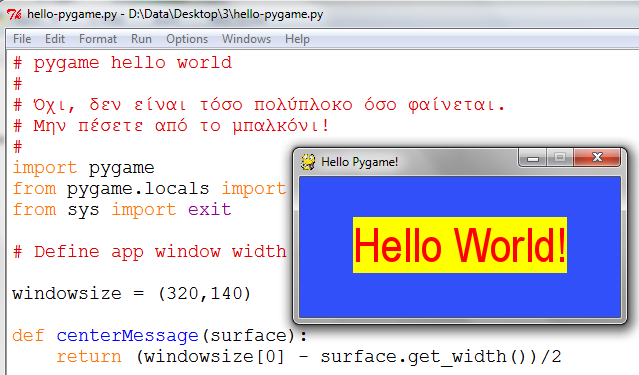
\includegraphics[width=0.5\textwidth]{images/chapter4/hello}
  \caption[Hello World σε Pygame]{To hello-world σε pygame. Ναι το ξέρουμε ότι δείχνει μεγάλο, αλλά κάνει πολύ περισσότερα πράγματα από ότι φαίνεται με την πρώτη ματιά.}
  \label{4-2}
\end{SCfigure}

Ας το πάμε λοιπόν γραμμή -- γραμμή και ταυτόχρονα θα βλέπουμε τις νέες έννοιες όπως ο {\em αντικειμενοστραφής προγραμματισμός}, η {\em επεξεργασία συμβάντων (events)} και ο προγραμματισμός που οδηγείται από συμβάντα ({\em event driven programming}).

\begin{minted}[bgcolor=bg, frame=lines, framesep=10pt]{python}
import pygame
from pygame.locals import *
from sys import exit
\end{minted}

Με την πρώτη εντολή φυσικά δηλώνουμε τη χρήση της βιβλιοθήκης pygame. Καθώς φαντάζεστε ότι χρησιμοποιούμε από pygame θα ξεχωρίζει καθώς θα είναι της μορφής {\tt pygame.<εντολή>}. H δεύτερη εντολή χρήζει περαιτέρω ερμηνείας: το {\tt pygame.locals} περιέχει μια σειρά από συμβολικές σταθερές πολύ χρήσιμες όταν χρησιμοποιούμε το pygame. Για παράδειγμα δίνει ονόματα στους κωδικούς των πλήκτρων -- τους αριθμούς που επιστρέφει ο ελεγκτής πληκτρολογίου στο λειτουργικό καθώς χτυπάμε τα πλήκτρα στην απέλπιδη προσπάθεια μας να γλιτώσουμε το διαστημόπλοιο μας από τα εχθρικά πυρά! H {\tt from} μας επιτρέπει να κρατήσουμε ότι θέλουμε από ένα module -- βάζοντας * λέμε ότι θέλουμε ουσιαστικά να κάνουμε import τα πάντα ενώ ταυτόχρονα δεν χρειάζεται πλέον να βάζουμε από μπροστά το όνομα του module όταν χρησιμοποιούμε κάτι από αυτό. Αν τώρα αναρωτιέστε γιατί δεν το κάνουμε αυτό πάντα, σας το αφήνω σαν άσκηση.

 Το {\tt exit} από το module {\tt sys} το χρειαζόμαστε για να μπορούμε να τερματίσουμε όμορφα ένα πρόγραμμα. Σε μερικές πλατφόρμες (ονόματα δεν λέμε, windows δεν δείχνουμε) θα έχετε περίεργα μηνύματα λάθους και κολλήματα αν δεν καλέσετε την {\tt exit()} στο τέλος του προγράμματος σας.

\begin{minted}[bgcolor=bg, frame=lines, framesep=10pt]{python}
windowsize = (320,140)
\end{minted}

Το {\tt windowsize} είναι ένα tuple (θυμηθείτε, τα tuples μοιάζουν με τις λίστες αλλά έχουν κάποιους περιορισμούς) και περιέχει το μέγεθος (πλάτος, ύψος) του παραθύρου μας. Πολλές από τις συναρτήσεις του pygame δέχονται δεδομένα σε μορφή tuple.

Αφήνουμε για την ώρα την ερμηνεία της συνάρτησης {\tt centerMessage} (που πρέπει να φαντάζεστε τι κάνει αν έχετε μελετήσει το προηγούμενο κεφάλαιο) και {\tt getQuit} που θα δούμε μόλις κατανοήσουμε το κύριο μέρος του προγράμματος:


\begin{minted}[bgcolor=bg, frame=lines, framesep=10pt]{python}
def main():
  pygame.init()
\end{minted}

H {\tt init} είναι η πρώτη συνάρτηση του pygame που πρέπει να καλέσετε στην αρχή του προγράμματος σας για να αρχικοποιηθεί η λειτουργία του pygame.

\begin{minted}[bgcolor=bg, frame=lines, framesep=10pt]{python}
  surfacecolor = (50,80,250)
\end{minted}

Σε αυτό το tuple ορίζουμε το χρώμα της επιφάνειας μας, δίνοντας τιμές για τα χρώματα κόκκινο, πράσινο και μπλε αντίστοιχα. Ο συνδυασμός δίνει ένα ενδιαφέρον γαλαζοπράσινο χρωματάκι που θα είναι το φόντο μας.

\begin{minted}[bgcolor=bg, frame=lines, framesep=10pt]{python}
  screen = pygame.display.set_mode(windowsize, DOUBLEBUF)
\end{minted}

Το παραπάνω δημιουργεί την βασική μας επιφάνεια {\tt screen}: το παράθυρο που μέσα σε αυτό θα εμφανιστούν τα πάντα. Παρατηρήστε ότι και το μέγεθος το δίνουμε σε μορφή tuple. To {\tt DOUBLEBUF} (μια συμβολική σταθερά που πήραμε από το {\tt pygame.locals}) αγνοήστε το για την ώρα, θα το συζητήσουμε λεπτομερειακά παρακάτω.

\begin{minted}[bgcolor=bg, frame=lines, framesep=10pt]{python}
  pygame.display.set_caption("Hello Pygame!")
\end{minted}

Ο τίτλος του παραθύρου. Ξέρετε, αυτό το ενοχλητικό κείμενο που εμφανίζεται στην μπάρα του παραθύρου και μας εκνευρίζει την ώρα που προσπαθούμε να μετακινήσουμε το παράθυρο με το ποντίκι μας.

\begin{minted}[bgcolor=bg, frame=lines, framesep=10pt]{python}
  textfont = pygame.font.SysFont("Arial",48)
\end{minted}

Εδώ δημιουργούμε ένα αντικείμενο font. Για να το απλουστεύσουμε λίγο, ας πούμε ότι επιλέγουμε τη γραμματοσειρά με την οποία θα εμφανιστεί το κείμενο.

\begin{minted}[bgcolor=bg, frame=lines, framesep=10pt]{python}
  thetext = textfont.render("Hello Pygame!", True, (255,0,0),(255,255,0))
\end{minted}

Εδώ δημιουργούμε την επιφάνεια {\tt thetext} που περιέχει τη φράση Hello Pygame! Τα δύο tuples που βλέπετε αντιστοιχούν στο χρώμα προσκηνίου (foreground) και παρασκηνίου (background) αντίστοιχα. Πολύ απλά, κόκκινα γράμματα πάνω σε κίτρινο φόντο. Το {\tt True} ενεργοποιεί το {\em antialiasing} και θα μπορούσατε κάλλιστα να δοκιμάσετε και με {\tt False} για να δείτε τι σας πάει καλύτερα στο μάτι.

Έχουμε όμως ήδη αναφέρει τις λέξεις ``επιφάνεια'' και ``αντικείμενο'' και δεν τις έχουμε ερμηνεύσει. Στο pygame ότι θέλουμε να εμφανίσουμε το δημιουργούμε πάνω σε μια {\em επιφάνεια}. Μπορούμε να βάλουμε μια επιφάνεια πάνω σε μια άλλη. Η πρώτη μας επιφάνεια είναι το παράθυρο μας, στη μεταβλητή {\tt screen}. Μια δεύτερη επιφάνεια (που θα φροντίσουμε να μπει πάνω στην πρώτη) είναι αυτή που περιέχει το μήνυμα μας και αποθηκεύσαμε στη μεταβλητή {\tt thetext}.

Σας βλέπω να ρωτάτε τι είδους μεταβλητές είναι αυτές οι {\tt screen}, {\tt thetext}, {\tt thefont}. Μέχρι στιγμής έχετε δει μεταβλητές που περιέχουν strings, λίστες, αριθμούς. Τι ακριβώς είναι μια μεταβλητή που κρατάει μια επιφάνεια ή ένα font;

Καλό ερώτημα. Επιτρέψτε μου λοιπόν να σας εισάγω στον κόσμο των αντικειμένων και του αντικειμενοστραφούς προγραμματισμού! Ναι, πρόκειται για {\em αντικείμενα ή objects}. Σε σχέση με τον κλασικό προγραμματισμό ο αντικειμενοστραφής χρησιμοποιεί την έννοια του {\em αντικειμένου} για να αναφέρεται σε δομές που μεταξύ άλλων διαθέτουν {\em ιδιότητες ή χαρακτηριστικά (attributes ή properties)} καθώς και δικές τους συναρτήσεις για να χειρίζονται τα δεδομένα τους. Ξαναδείτε για παράδειγμα τη γραμμή:

\begin{minted}[bgcolor=bg, frame=lines, framesep=10pt]{python}
  thetext = textfont.render("Hello World!", True, (255,0,0),(255,255,0))
\end{minted}

Ένα αντικείμενο της κλάσης font διαθέτει την --- όπως την αποκαλούμε --- μέθοδο {\tt render} την οποία καλούμε. H {\tt render} δεν είναι μια συνάρτηση γενικής χρήσης που απλά χρησιμοποιεί το {\tt textfont} ως μια ακόμα παράμετρο. Αν ήταν, θα την καλούσαμε  κάπως έτσι:

\begin{minted}[bgcolor=bg, frame=lines, framesep=10pt]{python}
  thetext = render(textfont, "Hello World!", True, (255,0,0),(255,255,0))
\end{minted}

Η {\tt render} είναι μια συνάρτηση που ορίζεται για  την κλάση των αντικειμένων font και καλείται όπως βλέπετε με τον τρόπο:

\begin{verbatim}
αντικείμενο.ΌνομαΜεθόδου(παράμετροι_αν_υπάρχουν)
\end{verbatim}

Μάλιστα η συγκεκριμένη μέθοδος επιστρέφει ένα αντικείμενο που ανήκει στην κλάση επιφάνειας (surface). Κάθε κλάση μπορεί να περιέχει τις δικές της μεθόδους -- θα μάθετε λεπτομέρειες για τα αντικείμενα και τον αντικειμενοστραφή προγραμματισμό στο επόμενο κεφάλαιο.

Όσοι δεν φάγατε το σοκολατάκι που αναφέραμε προηγουμένως μάλλον είναι ώρα να το φάτε τώρα. Όσοι το φάγατε, κρύψτε τα για να μη φάτε όλο το κουτί. Θα  πάθετε ζάχαρο!

\begin{minted}[bgcolor=bg, frame=lines, framesep=10pt]{python}
  textx = centerMessage(thetext)
  texty = 40
\end{minted}

Για να εμφανιστεί το κείμενο, πρέπει να αποφασίσουμε τις συντεταγμένες του. Καθώς καταλαβαίνετε σε ένα παράθυρο γραφικών οι γραμμές και οι στήλες αναφέρονται σε pixels. Σε αντίθεση βέβαια με την κονσόλα κειμένου όπου η ελάχιστη θέση είναι ο ένας χαρακτήρας. Η γραμμή λοιπόν εδώ είναι το {\tt texty} ενώ το {\tt textx} υπολογίζεται από τη centerMessage ώστε το μήνυμα να κεντραριστεί. Το (0,0) είναι στην πάνω αριστερή γωνία της οθόνης και οι τιμές αυξάνονται προς τα κάτω και δεξιά -- θα το δούμε αυτό καλύτερα όμως σε επόμενο παράδειγμα.

\begin{minted}[bgcolor=bg, frame=lines, framesep=10pt]{python}
  endprogram = False

  while not endprogram:
    screen.fill(surfacecolor)
    screen.blit(thetext,(textx,texty))
    endprogram = getQuit()
    pygame.display.update()

  pygame.quit()
  exit()
\end{minted}

Και επιτέλους φτάσαμε στο κύριο βρόχο του προγράμματος. Ας δούμε πρώτα λίγο τις εσωτερικές εντολές και μετά θα καταλάβετε γιατί μιλάμε για βρόχο, σε ένα πρόγραμμα που το μόνο που κάνει είναι να τυπώνει ένα μήνυμα!

\begin{minted}[bgcolor=bg, frame=lines, framesep=10pt]{python}
    screen.fill(surfacecolor)
\end{minted}

Αν έχετε πιάσει το νόημα, φαντάζεστε ότι ένα αντικείμενο τύπου επιφάνειας διαθέτει μια μέθοδο {\tt fill} με την οποία μπορούμε να το γεμίσουμε με χρώμα. Το χρώμα {\tt surfacecolor} θα γεμίσει την επιφάνεια {\tt screen} που αντιπροσωπεύει το παράθυρο μας.
Για να βάλουμε μια επιφάνεια πάνω σε μια άλλη, χρησιμοποιούμε τη μέθοδο {\tt blit}. Καλώντας:

\begin{minted}[bgcolor=bg, frame=lines, framesep=10pt]{python}
    screen.blit(thetext,(textx,texty))
\end{minted}

βάζουμε την επιφάνεια {\tt thetext} πάνω στην {\tt screen} στις συντεταγμένες {\tt textx, texty} (παρατηρήστε ότι και αυτές δίνονται σε μορφή tuple,  για αυτό και η παρένθεση).

\begin{minted}[bgcolor=bg, frame=lines, framesep=10pt]{python}
    pygame.display.update()
\end{minted}

Αυτό και αν είναι μυστήριο! Τι update; Πολύ απλά: ότι και αν κάνετε σε οποιαδήποτε επιφάνεια δεν γίνεται ορατό πριν καλέσετε την update. Γιατί πολύ απλά όλη αυτή η σχεδίαση, το γέμισμα με χρώμα, η επιφάνεια με το κείμενο που βάλατε πάνω από τη screen δεν έγιναν απευθείας στην μνήμη που αντιπροσωπεύει την οθόνη σας (τη RAM δηλ. της κάρτας γραφικών). Έγιναν σε μια άλλη, προσωρινή περιοχή μνήμης (buffer) η οποία αντιγράφεται πολύ γρήγορα στη μνήμη οθόνης. Έχετε δηλ. δημιουργήσει πλήρως το καρέ σας πριν το εμφανίσετε, αποφεύγοντας την πιθανότητα ο χρήστης της εφαρμογής σας να δει τα περιεχόμενα να σχεδιάζονται σιγά -- σιγά μπροστά του (και να κατηγορεί το πρόγραμμα σας ή το μηχάνημα του για χαμηλή ταχύτητα!). Και τώρα καταλαβαίνετε τι σημαίνει το {\tt DOUBLEBUF} που είδαμε πριν -- τις δύο περιοχές μνήμης που χρησιμοποιούμε για τη σχεδίαση της οθόνης μας!

\section{Event Driven Programming}
\label{section:event-driven-programming}
Αν έχετε γράψει ένα πρόγραμμα για παραθυρικό περιβάλλον (ακόμα και στη Visual Basic η οποία κρύβει πολλές λεπτομέρειες) θα ξέρετε ότι μια σημαντική διαφορά με μια εφαρμογή κονσόλας είναι ο χειρισμός των {\em συμβάντων, ή events}.

Οι εφαρμογές που γράφουμε στην κονσόλα δεν έχουν την έννοια των συμβάντων: εκτελούνται η μια εντολή μετά την άλλη και δέχονται είσοδο από το χρήστη μόνο όταν υπάρχει κάποια εντολή τύπου {\tt input}. Σε μια παραθυρική εφαρμογή όμως τα πράγματα είναι διαφορετικά. Τι γίνεται για παράδειγμα αν ξαφνικά ο χρήστης κάνει κλικ στο close (X) του παραθύρου; Ίσως πιστεύετε ότι το λειτουργικό χειρίζεται αυτές τις λειτουργίες αλλά δεν είναι ακριβώς έτσι. Απλά το λειτουργικό στέλνει ένα μήνυμα στην εφαρμογή σας ``Ο χρήστης πάτησε το close, μάλλον κάτι πρέπει να κάνεις για αυτό''. Η εφαρμογή σας πρέπει να είναι έτοιμη ανά πάσα στιγμή να επεξεργαστεί τα μηνύματα που δέχεται από το λειτουργικό -- αν δεν το κάνει και ο χρήστης εξακολουθεί να πατάει μανιωδώς το close, το λειτουργικό θα τερματίσει την εφαρμογή αφού πρώτα δείτε το γνωστό μήνυμα ``Δεν αποκρίνεται''. Εκτός φυσικά από τα μηνύματα που μας στέλνει το λειτουργικό θα πρέπει ανά τακτά διαστήματα να διαβάζουμε π.χ. και το πληκτρολόγιο με το οποίο κατευθύνουμε το παιχνίδι μας. Περισσότερα για αυτό θα δούμε σε επόμενα κεφάλαια.

Ναι λοιπόν, το πρόγραμμα μας τρέχει και εκτελείται ακόμα και μετά που θα τυπωθεί το μήνυμα ``Hello World!''. Αν τερμάτιζε εκεί, το παράθυρο θα έκλεινε πριν καλά καλά προλάβουμε να δούμε το μήνυμα. Το πρόγραμμα μας τερματίζει μόλις ο χρήστης πιέσει το close --- τότε λαμβάνεται το μήνυμα {\tt QUIT}:

\begin{minted}[bgcolor=bg, frame=lines, framesep=10pt]{python}
def getQuit():
  for event in pygame.event.get():
    if event.type == QUIT:
      return True
\end{minted}

Όλα τα συμβάντα που λαμβάνει το πρόγραμμα μας καταλήγουν σε ένα {\em queue} το ένα πίσω από το άλλο. Τα διαβάζουμε χρησιμοποιώντας την {\tt pygame.event.get()} η οποία δημιουργεί μια λίστα από events τα οποία επεξεργαζόμαστε ένα -- ένα με τη {\tt for}. Παρατηρήστε ότι στο συγκεκριμένο πρόγραμμα δεν ελέγχουμε για τίποτα άλλο εκτός από το {\tt QUIT} καθώς το πρόγραμμα μας είναι πολύ απλό.

Η επεξεργασία των events πρέπει να γίνεται συχνά. Παρατηρήστε ότι καλούμε την {\tt getQuit} σε κάθε κύκλο που κάνει ο βρόχος {\tt while}.

\begin{SCfigure}
  \centering
  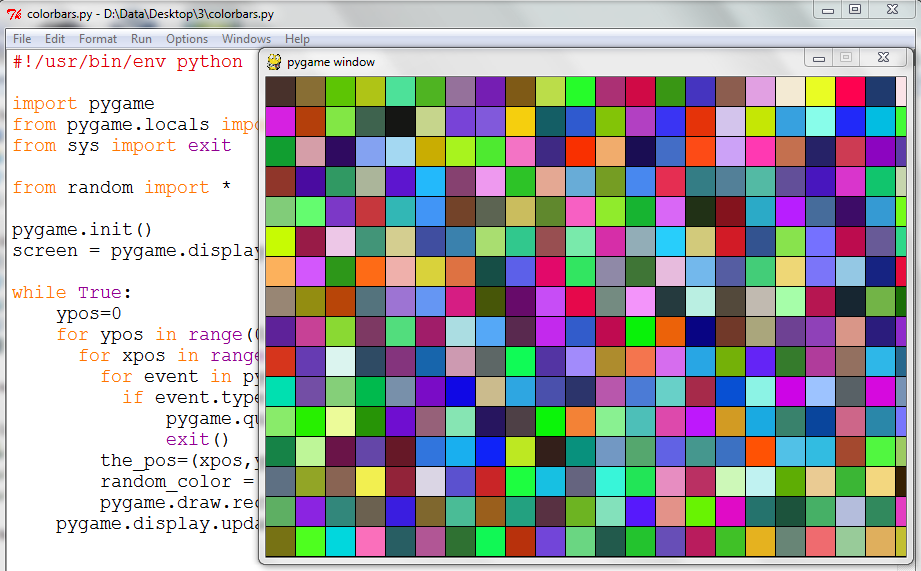
\includegraphics[width=0.5\textwidth]{images/chapter4/colorbars}
  \caption[Πρόγραμμα colorbars]{Αντιγράψτε αυτό το προγραμματάκι από το παράρτημα (σελ. \pageref{listing:colorbars}) και εκτελέστε το. Έπειτα αρχίστε τις παραλλαγές! Δοκιμάστε να αλλάξετε το μέγεθος των τετραγώνων, τις αποστάσεις μεταξύ τους ή και το σχήμα τους. Κάντε τα παραλληλόγραμμα ή κύκλους. Δείτε και στο \url{http://www.pygame.org/docs/ref/draw.html}  για βοήθεια σχετικά με τις εντολές σχεδίασης.}
  \label{4-6}
\end{SCfigure}

\section{Frames και Framerate}

Οι πιο παρατηρητικοί από εσάς θα είδατε ότι το κείμενο ``Hello World!'' τυπώνεται συνέχεια μέσα στο βρόχο while! Είναι απαραίτητο αυτό; Πόσες φορές το δευτερόλεπτο συμβαίνει; Τι θα γίνει αν μετακινήσουμε τις εντολές εμφάνισης έξω από το βρόχο και αφήσουμε σε αυτόν μόνο την επεξεργασία των συμβάντων;

Κάθε φορά που εκτελείται ο βρόχος, το πρόγραμμα μας εμφανίζει το μήνυμα στην οθόνη. Βέβαια το μήνυμα μας είναι στατικό και δεν βλέπουμε καμιά αλλαγή. Σε ένα παιχνίδι όμως κάθε εκτέλεση του βρόχου περιέχει κάποια αλλαγή --- κάποια κίνηση --- και δημιουργεί ένα {\em καρέ (frame)} του παιχνιδιού. Όσο πιο πολλά καρέ παράγονται σε ένα δευτερόλεπτο, τόσο πιο ομαλή είναι η κίνηση του παιχνιδιού. Τυπικά χρειαζόμαστε 50 καρέ το δευτερόλεπτο για να έχουμε τέλεια κίνηση.  Είναι αυτό που ονομάζουμε {\em framerate} και για το οποίο γίνεται πάντα τόσος λόγος σε όσους παίζουν παιχνίδια first person shooters (και ξοδεύουν αντίστοιχα εκατοντάδες ευρώ για κάρτες γραφικών).

\begin{figure}
  \centering
  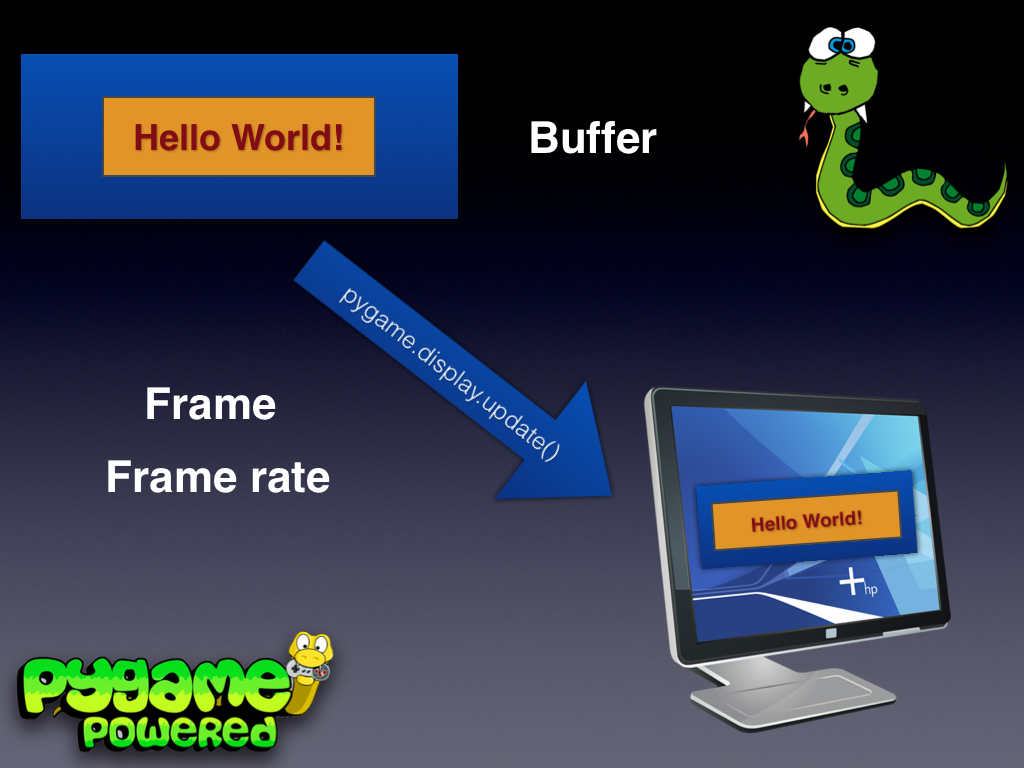
\includegraphics[width=0.8\textwidth]{images/chapter4/buffers}
  \caption[Buffering]{Μια εικόνα αξίζει όσο χίλιες λέξεις. Πως λειτουργεί το buffering, σχηματικά. Η οθόνη σχεδιάζεται στην ενδιάμεση μνήμη και με το update μεταφέρεται απευθείας στη μνήμη οθόνης.}
  \label{4-5}
\end{figure}

Τη δεδομένη στιγμή το ``παιχνίδι'' μας τρέχει με τόσα καρέ το δευτερόλεπτο όσα αντέχει ο υπολογιστής μας! Μπορούμε όμως στο pygame τόσο να μετρήσουμε το framerate που επιτυγχάνει το μηχάνημα μας (το οποίο είναι απαραίτητο όπως θα δείτε) όσο και να το περιορίσουμε σε ένα συγκεκριμένο αριθμό αν θέλουμε.

Και για να απαντήσω και στο άλλο ερώτημα σας, στο συγκεκριμένο πρόγραμμα πράγματι θα μπορούσατε να μετακινήσετε τις εντολές για το κείμενο έξω από το βρόχο. Αλλά είναι κάτι που δεν θα δείτε σε παιχνίδια!

\section{Bouncing Ball -- Επιτέλους Γραφικά και Κίνηση!}

Για να δούμε επιτέλους και λίγη κίνηση! Το πρόγραμμα που σας παρουσιάζουμε εδώ είναι το γνωστό bouncing ball:

\begin{minted}[bgcolor=bg, linenos, frame=lines, framesep=10pt]{python}
#
# Bouncing ball
#

import pygame
from pygame.locals import *
from sys import exit
\end{minted}

\begin{minted}[bgcolor=bg, linenos, firstnumber=8, frame=lines, framesep=10pt]{python}
def getQuit():
  for event in pygame.event.get():
    if event.type == QUIT:
      return True
  return False

def main():
  pygame.init()
  ballimage = 'soccer-ball.png'
  x,y = 100.0,100.0
  xspeed,yspeed = 50,50
  windowsize = (640,480)
  surfacecolor = (50,80,250)
  screen = pygame.display.set_mode(windowsize, DOUBLEBUF)
  ball = pygame.image.load(ballimage)
  ballwidth = ball.get_width()
  ballheight = ball.get_height()
  clock = pygame.time.Clock()

  # Uncomment the framerate line and change
  # time = clock.tick() in main loop to
  # time = clock.tick(framerate)
  # to limit the animation to a specific framerate

  #framerate = 30

  textfont = pygame.font.SysFont("Arial",24)
\end{minted}

\begin{minted}[bgcolor=bg, linenos, firstnumber=35, frame=lines, framesep=10pt]{python}
  #
  # Main loop
  #

  endprogram = False
  while not endprogram:
    screen.fill(surfacecolor)
    screen.blit(ball, (x, y))
    time = clock.tick()
    thetext = textfont.render(str(1000/time), True, (255,0,0),(255,255,0))
    screen.blit(thetext,(0,0))
    time = time / 1000.0
    distance_x = time * xspeed
    distance_y = time * yspeed
    x = x + distance_x
    y = y + distance_y

    if (x > (640.0-ballwidth) or x<=0.0):
      xspeed = -xspeed
    if (y > (480.0-ballheight) or y<=0.0):
      yspeed = -yspeed
    pygame.display.update()
    endprogram = getQuit()

  pygame.quit()
  exit()

if __name__ == "__main__":
  main()
\end{minted}

\begin{figure}
  \centering
  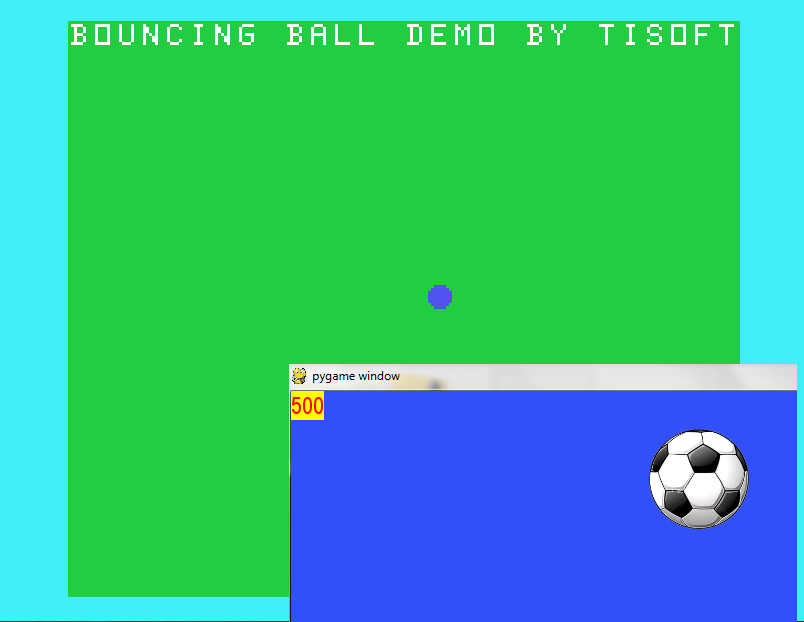
\includegraphics[width=0.8\textwidth]{images/chapter4/bounce1}
  \caption[Παλιό και νέο bouncing ball]{Το παλιό και το καινούριο: Μια εικόνα του πρωτότυπου bouncing ball,  όπως το έγραψα το 1985 στον TI-99/4A.  Είναι εμφανώς\ldots{} retro, αλλά φυσικά έχει πλάκα! Την εποχή εκείνη η κίνηση δεν γινόταν με καρέ (όπου συνήθως ξανασχεδιάζουμε όλη την οθόνη) αλλά με sprites ή κίνηση χαρακτήρων, όπου απλά μετακινούμε το αντικείμενο στη νέα του θέση και το σβήνουμε από την παλιά. Δεν θα ήταν άλλωστε δυνατόν για ένα μηχάνημα της εποχής να ανασχεδιάζει μια ολόκληρη οθόνη 50--60 φορές το δευτερόλεπτο. Και ούτε λόγος για\ldots{} double buffering!}
  \label{4-1}
\end{figure}

Για να δούμε μερικά ενδιαφέροντα σημεία:

\begin{minted}[bgcolor=bg, frame=lines, framesep=10pt]{python}
  x,y = 100.0,100.0
  xspeed,yspeed = 50,50
\end{minted}

Αρχική θέση της μπάλας και αρχική ταχύτητα στους δύο άξονες.

\begin{minted}[bgcolor=bg, frame=lines, framesep=10pt]{python}
  ballimage = 'soccer-ball.png'
  ball = pygame.image.load(ballimage)
\end{minted}

Φόρτωση της μπάλας από το αρχείο {\tt soccer-ball.png}. Δημιουργείται μια επιφάνεια (surface) που ανατίθεται στη μεταβλητή {\tt ball}.

\begin{minted}[bgcolor=bg, frame=lines, framesep=10pt]{python}
  ballwidth = ball.get_width()
  ballheight = ball.get_height()
\end{minted}

\begin{SCfigure}
  \centering
  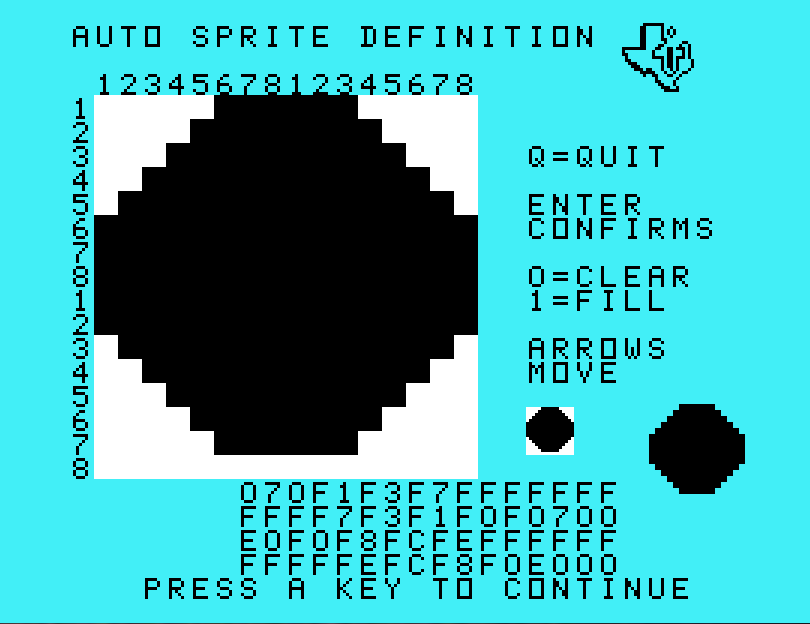
\includegraphics[width=0.4\textwidth]{images/chapter4/spritedefiner}
  \caption[Sprite definer]{Την παλιά καλή(;) εποχή, δεν υπήρχε το Internet
για να κατεβάσει κανείς την\ldots{} μπάλα της αρεσκείας του σε έτοιμο bitmap. Τα γραφικά σχεδιάζονταν στο χέρι (σε χαρτί με τετραγωνάκια!) ή σε προγράμματα που στις μέρες μας θα έμοιαζαν με icon editors. Και εννοείται ότι και αυτά τα προγράμματα τα γράφαμε μόνοι μας! Στη φώτο, το Auto Sprite Definition, μια δική μου εκδοχή σε ένα αντίστοιχο πρόγραμμα της Texas Instruments που επιτρέπει τη σχεδίαση κινούμενων γραφικών (sprites) για παιχνίδια.  Άπειρα pacman και διαστημοπλοιάκια έχουν σχεδιαστεί σε αυτό το πρόγραμμα!}
  \label{4-3}
\end{SCfigure}

Μπορούμε να ρωτήσουμε ένα αντικείμενο τύπου surface να μας πει τις
διαστάσεις του! Πρόκειται για τις μεθόδους {\tt get\_width()} και {\tt get\_height()}.

\begin{minted}[bgcolor=bg, frame=lines, framesep=10pt]{python}
  clock = pygame.time.Clock()
\end{minted}

Το παραπάνω δημιουργεί ένα αντικείμενο τύπου {\tt clock}. Μέσα στο βρόχο υπάρχει η εντολή:

\begin{minted}[bgcolor=bg, frame=lines, framesep=10pt]{python}
    time = clock.tick()
\end{minted}

Στη μεταβλητή {\tt time} θα βρείτε σε χιλιοστά δευτερολέπτου το χρόνο που πέρασε από την προηγούμενη φορά που εκτελέστηκε η εντολή. Καθώς εκτελείται μια φορά σε κάθε κύκλο του {\tt while}, μπορεί να χρησιμοποιηθεί για τον υπολογισμό του {\tt framerate = 1000 / time}.

Πρέπει τόσο στο γρήγορο, όσο και στο αργό μηχάνημα η μπάλα να κινείται με σταθερή ταχύτητα -- ανεξάρτητα από το framerate! Για να το επιτύχουμε πρέπει στη μονάδα του χρόνου (το 1 sec) η απόσταση που κινείται η μπάλα να είναι σταθερή. Σε ένα γρήγορο μηχάνημα η κίνηση θα είναι ωραία και ομαλή. Σε ένα αργό όμως θα φαίνεται να κάνει πηδηματάκια! Ωστόσο, η πραγματική ταχύτητα θα είναι ίδια. Πως γίνεται αυτό; Αν θυμηθείτε λίγο τη φυσική σας, για ομαλή κίνηση ο τύπος είναι:

\begin{verbatim}
Απόσταση = Ταχύτητα * Χρόνος
\end{verbatim}

(Ναι, τελικά η φυσική δεν είναι μόνο για να λύνετε ασκήσεις. Είναι και για να γράφετε παιχνίδια, αν και αυτό μάλλον παρέλειψαν να σας το πουν οι καθηγητές σας). Και αυτό ακριβώς κάνουμε και εμείς:

\begin{minted}[bgcolor=bg, frame=lines, framesep=10pt]{python}
    time = time / 1000.0
\end{minted}

Μετατροπή του χρόνου σε δευτερόλεπτα.

\begin{minted}[bgcolor=bg, frame=lines, framesep=10pt]{python}
    distance_x = time * xspeed
    distance_y = time * yspeed
\end{minted}

Υπολογισμός της απόστασης που κινήθηκε η μπάλα  στους δύο άξονες.

\begin{minted}[bgcolor=bg, frame=lines, framesep=10pt]{python}
    x = x + distance_x
    y = y + distance_y
\end{minted}

Υπολογισμός της νέας θέσης της μπάλας.

Και φυσικά αντιλαμβάνεστε ότι τα {\tt if} που ακολουθούν αναλαμβάνουν να αντιστρέψουν την ταχύτητα της μπάλας όταν χτυπήσει σε κάποιο τοίχωμα (δηλ. το border του παραθύρου!)

\begin{SCfigure}
  \centering
  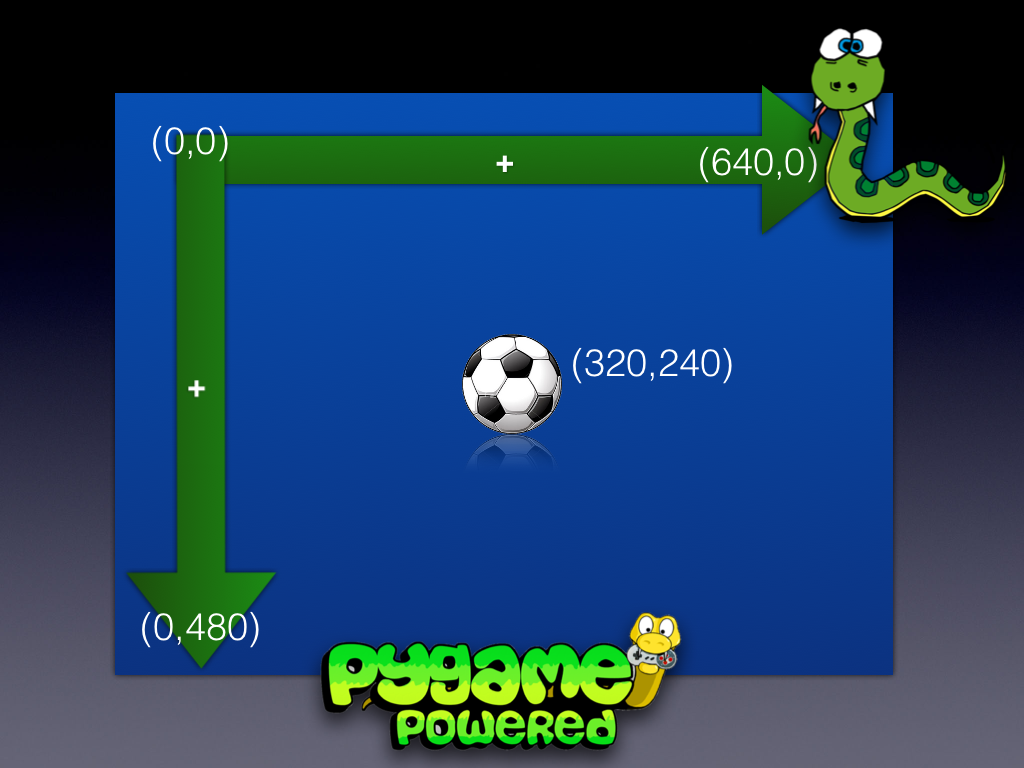
\includegraphics[width=0.5\textwidth]{images/chapter4/coordinates}
  \caption[Συντεταγμένες γραφικών]{Οι συντεταγμένες ξεκινάνε από το (0,0) στην πάνω αριστερή γωνία της οθόνης και αυξάνονται προς τα δεξιά και προς τα κάτω. Σε ένα παράθυρο μεγέθους 640Χ480, μια μπάλα στη μέση θα βρίσκονταν στις συντεταγμένες (320,240).}
  \label{4-4}
\end{SCfigure}

Το ενδιαφέρον είναι ότι το ``παιχνίδι'' μας τυπώνει το framerate στην οθόνη, με την εντολή:

\begin{minted}[bgcolor=bg, frame=lines, framesep=10pt]{python}
    thetext = textfont.render(str(1000/time), True, (255,0,0),(255,255,0))
    screen.blit(thetext,(0,0))
\end{minted}

Όσο πιο γρήγορος είναι ο υπολογιστής σας και η κάρτα γραφικών σας, τόσο μεγαλύτερος ο αριθμός που θα δείτε. Μπορούμε όμως να τον περιορίσουμε. Βγάλτε τo σχόλιο από τη γραμμή:

\begin{minted}[bgcolor=bg, frame=lines, framesep=10pt]{python}
  framerate = 30
\end{minted}

και αλλάξτε μέσα στο βρόχο την εντολή {\tt tick} ώστε να δείχνει:

\begin{minted}[bgcolor=bg, frame=lines, framesep=10pt]{python}
    time = clock.tick(framerate)
\end{minted}

Η γραμμή {\tt time} τώρα θα προκαλεί όση καθυστέρηση χρειάζεται ώστε το πρόγραμμα σας να εκτελείται με το συγκεκριμένο framerate! Δοκιμάστε με διαφορετικούς αριθμούς για να δείτε το αποτέλεσμα. Πάνω από 60 καρέ το δευτερόλεπτο ίσως να μη βλέπετε αισθητή διαφορά. Αλλά σε χαμηλά framerates θα βλέπετε κακή ποιότητα κίνησης. Η ταχύτητα όμως της μπάλας θα είναι ίδια.

Σαν άσκηση, δοκιμάστε το πρόγραμμα με διαφορετικές ταχύτητες μπάλας και framerates. Μετατρέψτε το ώστε να κινούνται δύο μπάλες αντί για μία! (Hint: μπορείτε να κάνετε blit το ίδιο surface σε δύο διαφορετικές θέσεις) Όταν οι δύο μπάλες συναντιούνται στην οθόνη, κάποια περνάει πάνω από την άλλη. Ποια και γιατί; Μπορείτε να το βρείτε;

Σας αφήνω τώρα να παίξετε και σας προκαλώ να γράψετε τα δικά σας απλά προγραμματάκια animation με βάση αυτά που είδατε μέχρι τώρα.

Θα βρείτε τα προγράμματα αυτής της ενότητας στο Παράρτημα: Hello Pygame σελ. \pageref{listing:hello-pygame}, Colorbars σελ. \pageref{listing:colorbars}, Bouncing Ball σελ. \pageref{listing:bouncing-ball}.
